\documentclass[]{article}
\usepackage{amsmath}
\usepackage{amssymb}
\usepackage{verbatim} %con verbatim escribes bloques de texto con letra mono.
\usepackage{graphicx} %para insertar imagenes, cuando meta yo una usa el codigo de ejemplo
\usepackage{listings}
\usepackage{fullpage}
\usepackage{color}
\usepackage{fancyvrb}
\usepackage[spanish]{babel}
\usepackage[utf8]{inputenc} %Para usar acentos directamente en latex
\usepackage{hyperref} %Para que el indice tenga hiperenlaces y si quieres poner los tuyos
\hypersetup{%
	pdfborder = {0 0 0}
}

\definecolor{mygreen}{rgb}{0,0.6,0}
\definecolor{mygray}{rgb}{0.5,0.5,0.5}
\definecolor{mymauve}{rgb}{0.58,0,0.82}

%Para insertar código: crea un recuadro con texto mono y lineas enumeradas. Puedes referenciar un fichero y no copiar y pegar aquí.
\lstset{ %
	backgroundcolor=\color{white},   % chohttp://xdxd.com/ose the background color; you must add \usepackage{color} or \usepackage{xcolor}
	basicstyle=\footnotesize,        % the size of the fonts that are used for the code
	breakatwhitespace=false,         % sets if automatic breaks should only happen at whitespace
	breaklines=true,                 % sets automatic line breaking
	captionpos=b,                    % sets the caption-position to bottom
	commentstyle=\color{mygreen},    % comment style
	frame=single,                    % adds a frame around the code
	keepspaces=true,                 % keeps spaces in text, useful for keeping indentation of code (possibly needs columns=flexible)
	numbers=left,                    % where to put the line-numbers; possible values are (none, left, right)
	numbersep=5pt,                   % how far the line-numbers are from the code
	numberstyle=\tiny\color{mygray}, % the style that is used for the line-numbers
	rulecolor=\color{black},         % if not set, the frame-color may be changed on line-breaks within not-black text (e.g. comments (green here))
	showspaces=false,                % show spaces everywhere adding particular underscores; it overrides 'showstringspaces'
	showstringspaces=false,          % underline spaces within strings only
	showtabs=false,                  % show tabs within strings adding particular underscores
	stepnumber=1,                    % the step between two line-numbers. If it's 1, each line will be numbered
	stringstyle=\color{mymauve},     % string literal style
	tabsize=4,
	inputencoding=utf8,
	title=\lstname                   % show the filename of files included with \lstinputlisting; also try caption instead of title
}

\usepackage{pdfpages}

\title{Computación Móvil}
\author{José Luis Cánovas Sánchez - 48636907A\\Ezequiel Santamaría Navarro - 20096517Z}

\begin{document}

\maketitle


\tableofcontents

\section{Manual de usuario}

Partimos de que tenemos una cuenta de usuario, se pueden usar de ejemplo una de las cuentas (se recomienda \textit{joseluis}):

\begin{verbatim}
Nombre - Login - Contraseña:
José Luis -joseluis - plisu
Ezequiel - ezequiel - memelord
\end{verbatim}

Cuando abrimos la app por primera vez se nos pide introducir el login único y contraseña de nuestra cuenta.

\hfill

Si no iniciamos sesión en otro dispositivo, la app no nos volverá a pedir iniciar sesión, pues usará el token único conseguido en el paso anterior, que \textit{\textbf{almacena en la memoria del dispositivo}}.

\hfill

Se nos mostrará una pantalla con la lista de conversaciones que tenemos con otros usuarios, (al inicio ninguna), y un botón para añadir una conversación nueva.

\begin{center}
	 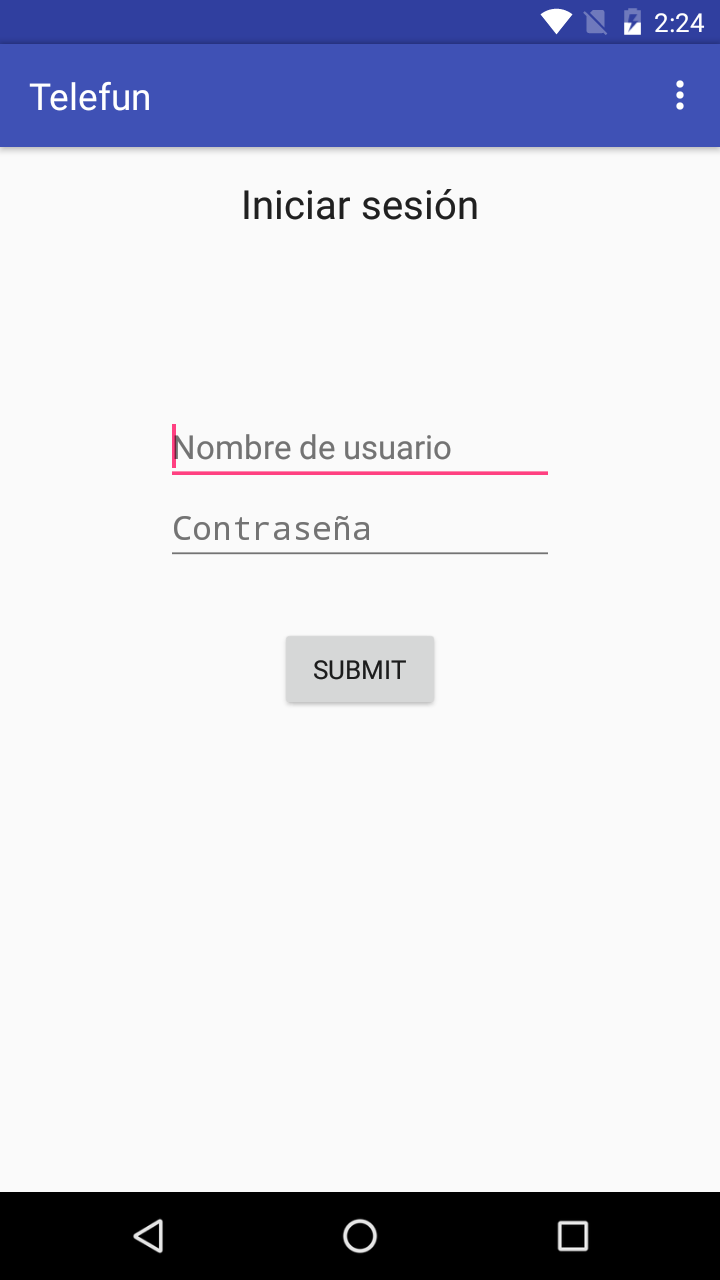
\includegraphics[width=0.35\linewidth]{images/login.png}
	 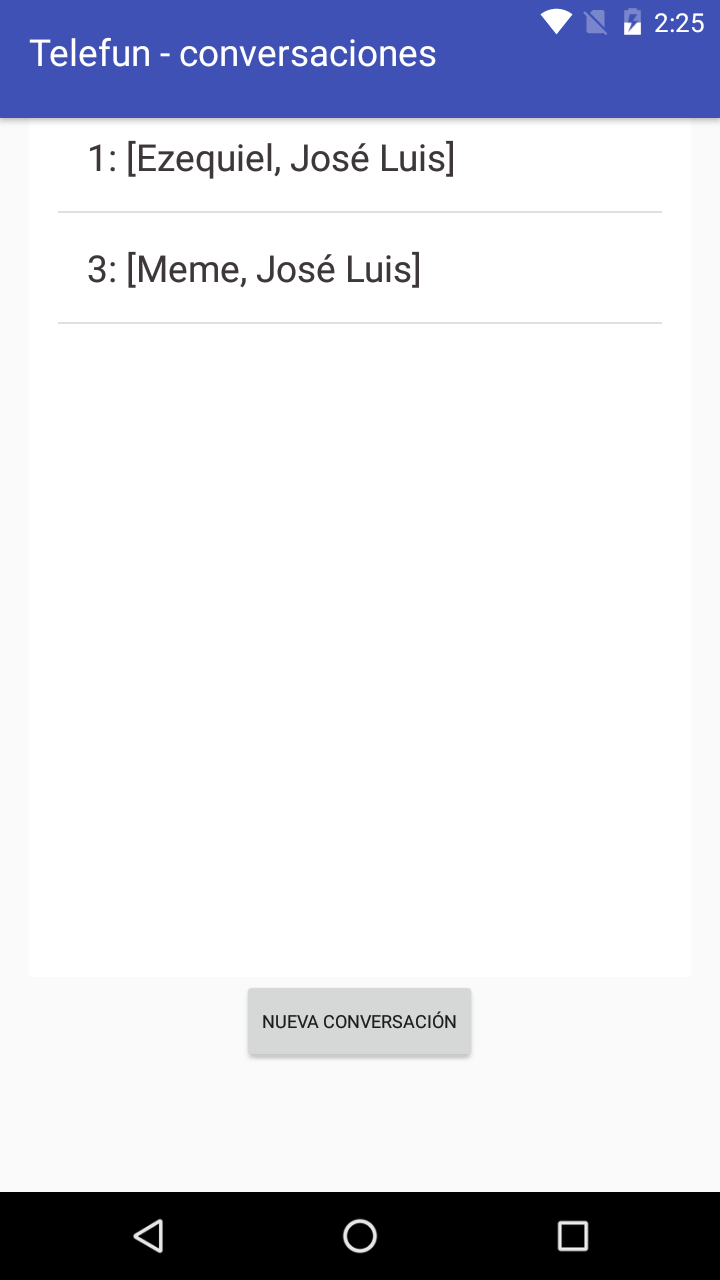
\includegraphics[width=0.35\linewidth]{images/listaconversaciones.png}
\end{center}

\hfill


Si pulsamos en el botón, nos llevará a la agenda de contactos, mostrando un campo de búsqueda y la lista de usuarios (inicialmente vacía).

Para \textbf{añadir un contacto}, se necesita un consentimiento mutuo, es decir, ambos usuarios deben indicar que quieren añadir al otro, y entonces podrán iniciar conversaciones. Para facilitar la prueba, por defecto el usuario \textit{ezequiel} ya envió la petición de contacto a \textit{joseluis}. Para que \textit{joseluis} la acepte, debe escribir en el campo de texto el \textit{login} de \textit{ezequiel} y pulsar \textit{intro}. Se envía automáticamente la petición al servidor, y volviendo a entrar en la lista de contactos, en ambos móviles aparecerá el otro usuario.


\begin{center}
	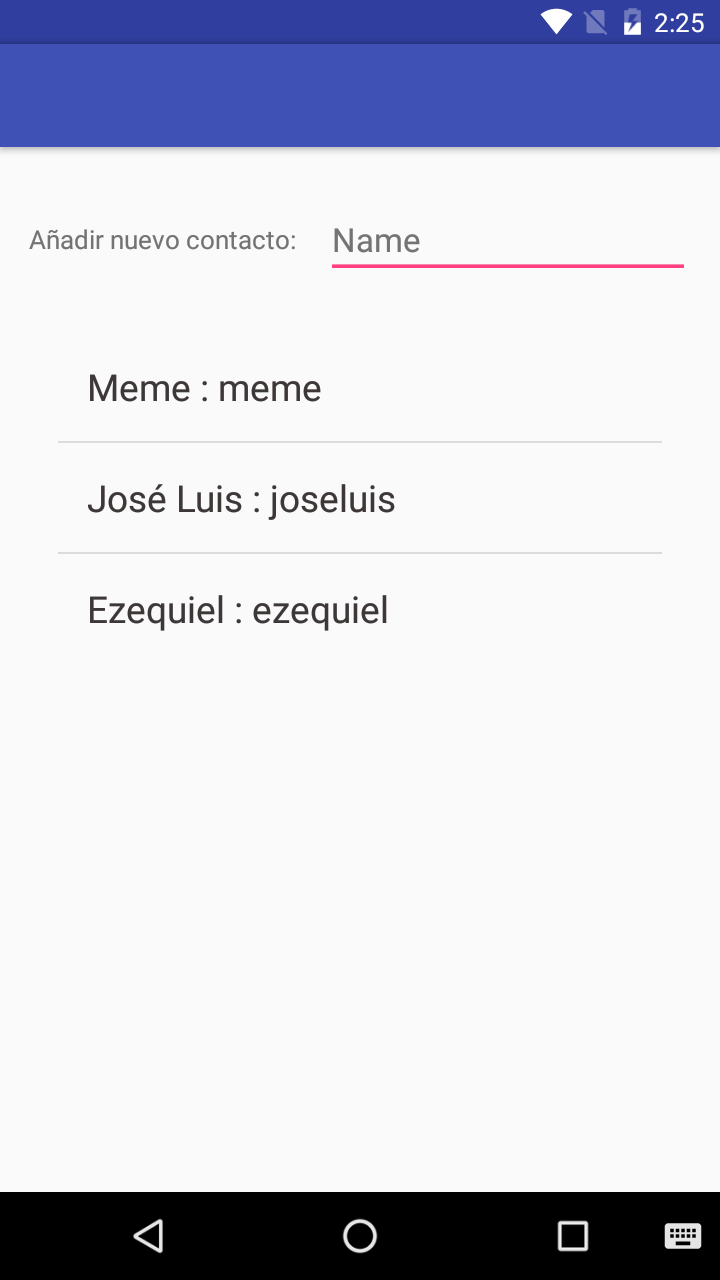
\includegraphics[width=0.35\linewidth]{images/agendacontactos.png}
\end{center}

\hfill

Para \textbf{añadir una conversación}, basta pulsar sobre un contacto de la agenda. Se mostrará un Toast indicando que se ha creado la conversación (o un error si no se pudo completar la petición con el servidor). Volviendo a la lista de conversaciones se mostrará la conversación creada. Pulsando sobre ella nos llevará a la vista del chat.

\hfill

En la vista del chat tenemos la conversación, un campo de texto para enviar mensajes cuando pulsamos \textit{intro} y un botón de compartir nuestra localización.

\begin{center}
	 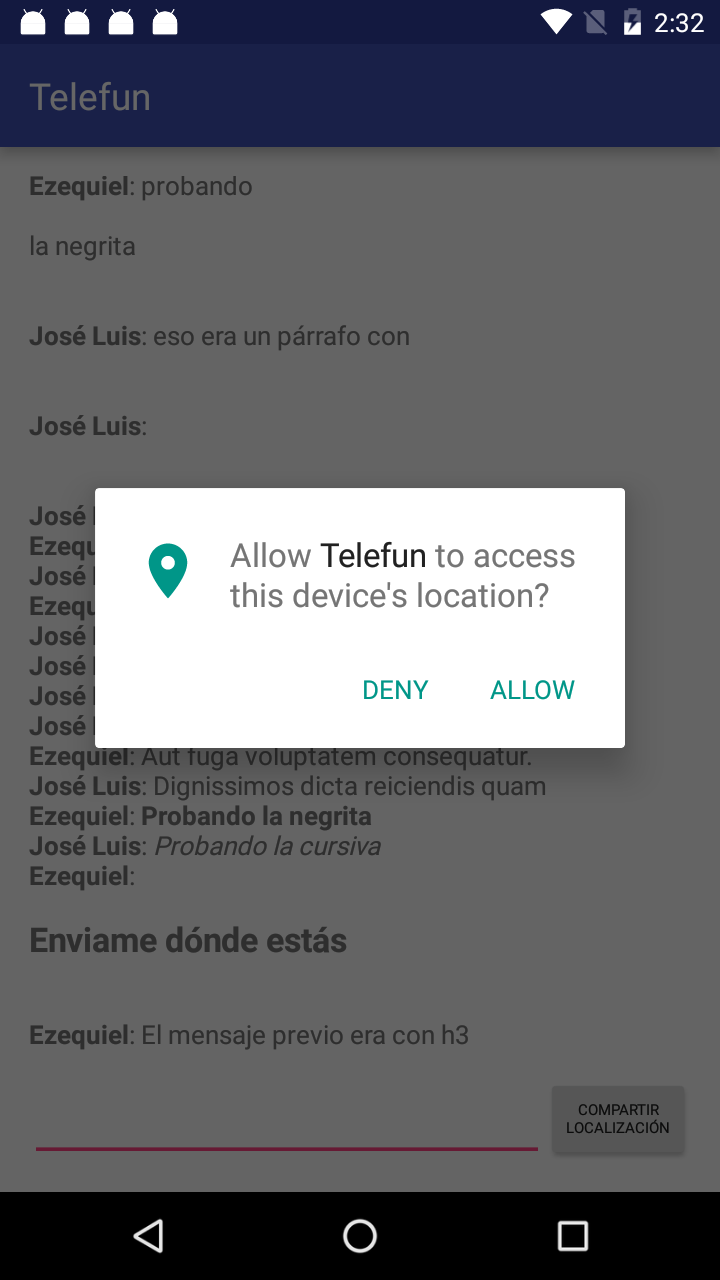
\includegraphics[width=0.35\linewidth]{images/localizacion.png}
	 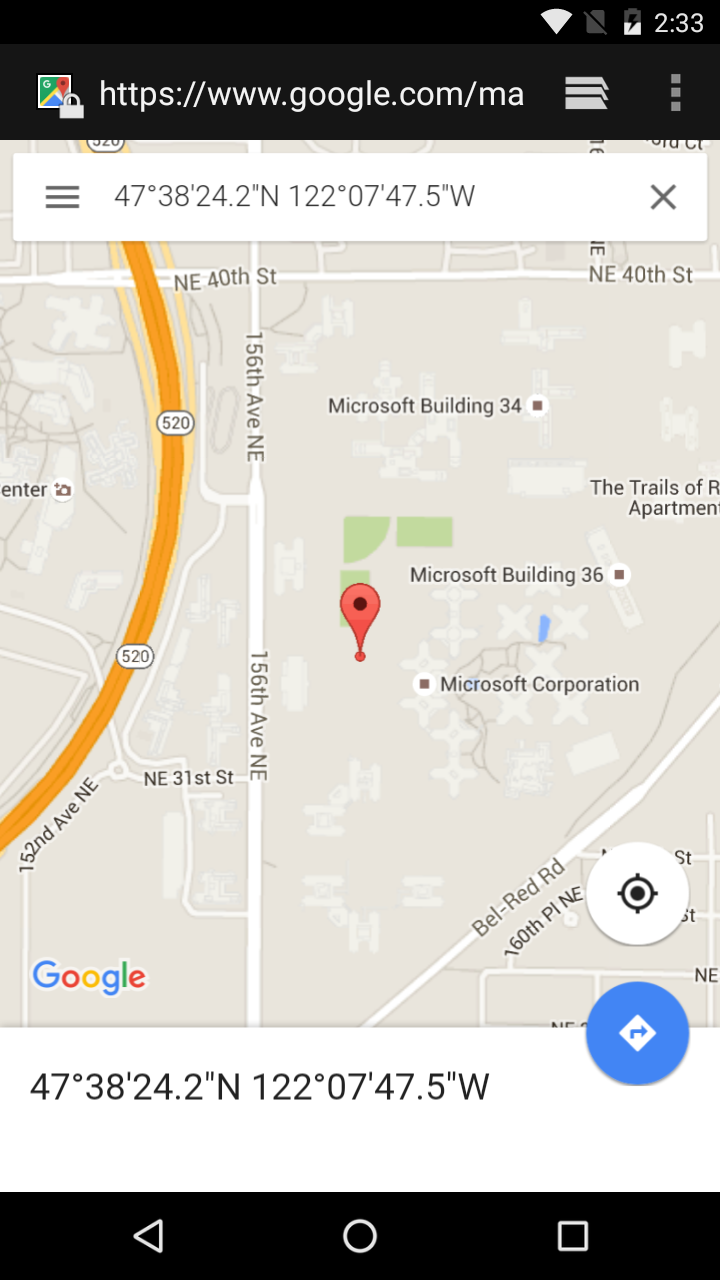
\includegraphics[width=0.35\linewidth]{images/map.png}
\end{center}

\hfill

En el campo de texto podemos escribir html básico, lo que nos permite, como en las últimas actualizaciones de Whatsapp, usar negrita, cursiva, escribir enlaces, etc.

El botón de compartir localización, la primera vez nos pedirá dar permiso a la app para acceder al GPS. Una vez dado, si pulsamos el botón se mandará un mensaje por el chat con el texto \textbf{\underline{Mapa}}, que al pulsar nos llevará a Google Maps con las coordenadas del móvil.

\hfill

Existe un servicio en segundo plano que sincroniza todas las conversaciones con el servidor cada 3.5 segundos, esté la app en primer o segundo plano, y se nos muestra una notificación con cada nuevo mensaje que nos llegue de otra persona. Si pulsamos en la notificación, se nos llevará a la lista de conversaciones de la app.

\begin{center}
		 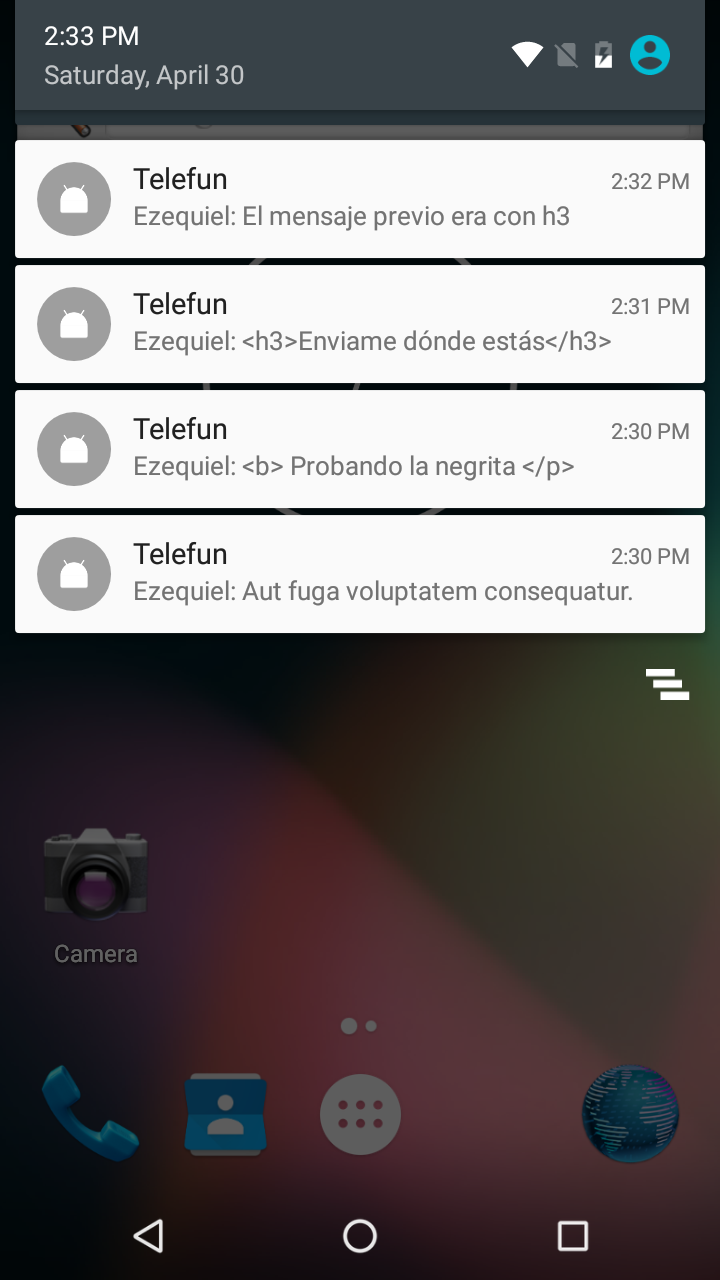
\includegraphics[width=0.35\linewidth]{images/notifications.png}
\end{center}


\hfill

Como todas las comunicaciones con el servidor se realizan por HTTPS, ningún elemento intermedio podría interceptar las comunicaciones.


\section{Diseño e implementación}


Telefun se basa en un servidor centralizado que almacena a los usuarios y sus datos, lista de contactos y conversaciones. Los clientes se conectan al servidor por HTTP/REST, usando para identificarse un token único para cada usuario. Esto permite que las conversaciones se puedan ver por cualquier app que implemente los mensajes HTTP/REST o por un navegador web.

Por esta estructura de servidor centralizado y acceso a las conversaciones por múltiples dispositivos, llamamos a la aplicación \textit{Telefun}, al ser más del estilo de \textit{Telegram} que de \textit{Whatsapp}.

Se detallan las características de la app y del servidor en las secciones siguientes, donde se irán mencionando cómo se han implementado las mejoras:
\begin{itemize}
	\item Geo-localización de usuarios.
	\item Persistencia de conversaciones y de la agenda de contactos del usuario.
	\item Recepción de notificaciones cuando lleguen mensajes, aunque la aplicación no se encuentre en primer plano.
	\item Securización de los mensajes intercambiados.
\end{itemize}


\subsection{Consideraciones por falta de dispositivo físico}

Debido a que ninguno de los dos tenemos un móvil Android, debemos utilizar máquinas virtuales, con las limitaciones que conlleva. Listamos algunas simplificaciones realizadas por ello:

\begin{itemize}
	\item Agenda de contactos: no sincronizamos con la agenda del dispositivo, pues tendríamos que rellenarla de cero en las mv. Utilizamos una agenda propia del servidor.
	\item No implementamos VoIP ni multimedia: el acceso de las máquinas virtuales a la cámara y micrófono depende del equipo donde se ejecuten y la estabilidad de la mv. Debido a que no podíamos confiar en que funcionaran con cada prueba, decidimos enfocarnos en otras mejoras de la app.
\end{itemize}

\subsection{Arquitectura de la aplicación}

En la siguiente sección mostramos el diagrama de clases de la aplicación.

\hfill

Existen dos interfaces básicas que implementan varias clases: \textit{OnAPIUpdate} y \textit{OnDataLoaded}. La primera se utiliza para comunicar entre sí las clases asíncronas que realizan conexiones al servidor, con las que esperan el contenido de la respuesta. La segunda sirve para comunicar las clases que deben procesar las respuestas y pueden depender de otra que haga conexiones asíncronas.

Por ejemplo, OnAPIUpdate lo implementa \textit{TelefunActivity} para comprobar con un GET si el token es correcto, usando \textit{RetrieveURLwithToken}. Si tras la conexión HTTP se recibe una respuesta de éxito, \textit{RetrieveURLwithToken} llamará a Telefun.OnSuccess(), y si es de fallo, a Telefun.OnError().

En el caso de OnDataLoaded, podemos ver \textit{Message} y \textit{Contact}. \textit{Message} depende de que un contacto tenga descargada su información para asegurar que el \textit{creador} existe, por ello, es un listener de \textit{Contact}. Cuando se pide un contacto a \textit{Contact}, éste puede necesitar conectarse al servidor para descargar su información, y una vez la tiene, llama a Message.OnLoad() para avisar que tiene toda la información y la puede usar.

\hfill

\hfill

La ejecución empieza en el \textit{Activity} \textit{TelefunActivity}, que se encarga de mostrar la ventana de login, guardar en memoria el token obtenido para futuros usos, comprobar que es válido, y llevarnos a la lista de conversaciones.

\hfill


En \textit{ListConversationsActivity} se llama a la clase \textit{ConversationsCatalog} para que sincronice las nuevas conversaciones con el servidor, y cuando termina de descargar y tratar la información, al implementar \textit{OnDataLoaded} le avisan al llamar al método OnLoad(), que mostrará la lista de conversaciones con los participantes.

\hfill

Al ir a \textit{ChatActivity}, pasamos como parámetro extra (con \textit{intent.putExtra()}) el id de la conversación, único en el servidor, y que ya descargamos en la sincronización previa. Este activity muestra la lista de mensajes usando html para formatearlos, y ofrece el botón para compartir la localización.

Cuando se envía un mensaje, se pasa a la clase \textit{Conversation} que se encargará de enviar el POST al servidor, y se \textit{fuerza} un rebind de la conversación, para no esperar al servicio que lo hace cada 3.5 segundos.

\hfill

Hasta aquí hemos visto la interfaz a seguir hasta un chat. Internamente tenemos el paquete de \textit{messaging} que maneja los objetos con los datos y las comunicaciones al servidor.

Tenemos una clase catálogo de las conversaciones, una clase para almacenar una conversación, con sus participantes y mensajes, ambos objetos de las clases Contact y Message. Con estas clases tenemos representados todos los datos que nos puede dar el servidor: usuarios, conversaciones y mensajes.

Cuando se recuperan nuevos mensajes que nos envía otro usuario, se crea una notificación con el autor y contenido del mensaje, usando la clase \textit{TelefunNotificationManager}.

\hfill

En \textit{NewConversationActivity} tenemos la agenda de contactos y la posibilidad de crear nuevas conversaciones. Para ello utiliza una clase auxiliar \textit{ContactsSync} que sincroniza la lista de contactos y manda peticiones de nuevos contactos. De este modo evitamos tener que conocer el tipo de JSON que devuelve el servidor. Sin embargo, al crear una conversación, no es necesario almacenar el id de respuesta, pues en \textit{ListConversationsActivity}, la sincronización forzará recuperar el id del servidor. Por ello, el POST de nueva conversación lo hace directamente este activity.

\hfill

Por último el servicio de sincronización, implementado como un \textit{IntentService}, puede ejecutarse tanto en primer como en segundo plano, y fuerza que se actualicen todas las conversaciones (un rebind) cada 3.5 segundos. En resumen, un pulling al servidor para recuperar nuevos mensajes.

\hfill



\subsubsection{Diagrama de clases}

Se incluye en la página a continuación el diagrama de clases de la implementación de la app. Por razones de espacio, la página en pdf es más larga que el resto y se recomienda verlo por ordenador.

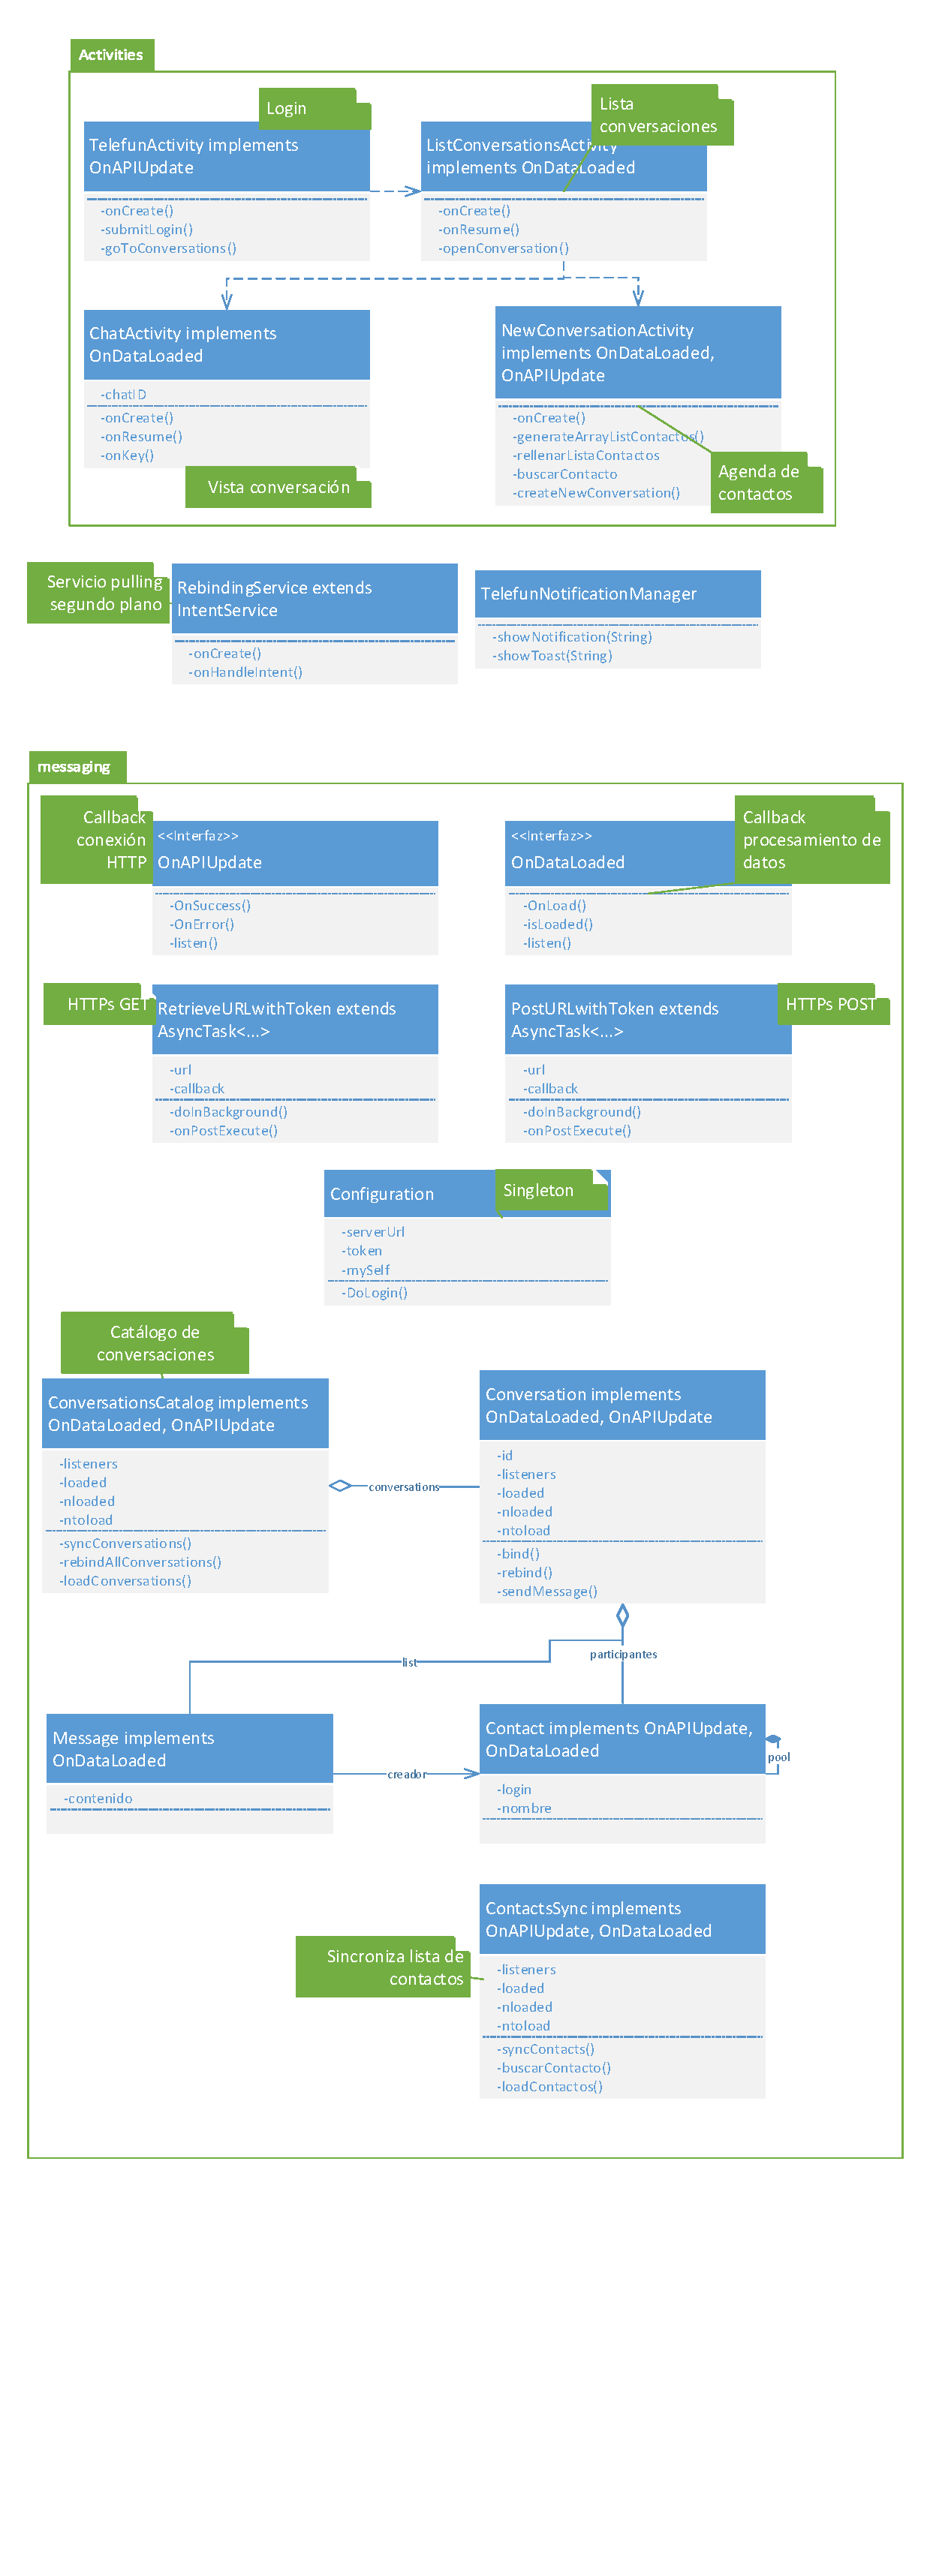
\includepdf[pages=-,fitpaper=true]{DiagramaClases.pdf}

\subsection{Servidor REST}

El servidor guarda en estructuras JSON toda la información: de los contactos, su nombre, login único y contraseña, lista de contactos y conversaciones. Para poder hacer llamadas HTTP/REST válidas, los mensajes GET y POST deben ir acompañados de una Cookie \textit{token}, con el valor del token único generado en el último inicio de sesión del usuario con su login y contraseña.

Para conseguir el token, un usuario debe hacer una petición del tipo

 \textit{urlServidor/usuarios/:usuario/token?password=:contraseña}
 
  donde \textit{:usuario} se debe sustituir por el login único del usuario, y \textit{:contraseña} por su contraseña. Esta llamada devuelve un token en forma de \textit{Set-Cookie} que se debe guardar en la app para evitar tener que insertar de nuevo el login y contraseña. Si se realiza el inicio de sesión en otro dispositivo, se genera un nuevo token y por seguridad no se aceptan los token antiguos, por lo que en la app se cerrará la sesión.

\hfill

Como servidor estamos usando el servicio \textit{Bluemix} de IBM, el cual nos automatiza el conseguir un certificado para que funcione el HTTPS sin tener que crear nuestra propia PKI.

\hfill

Al usar \textbf{HTTPS} junto a los \textbf{token} de usuario, en el intercambio de todos los mensajes con el servidor, conseguimos otra de las funcionalidades, \textbf{\textit{securización de los mensajes intercambiados}}. Y por el hecho de guardar todo en el servidor, conseguimos la \textbf{\textit{persistencia de conversaciones y de contactos del usuario}} no sólo en la app, sino en todos los clientes donde iniciemos sesión.

\hfill

Una vez hemos iniciado sesión y obtenemos el token, estos son los mensajes que se pueden intercambiar con el servidor:

\begin{itemize}
	\item get /usuarios/:usuario
	
	Devuelve en JSON los datos de contacto públicos de un usuario:
	
	\begin{BVerbatim}
	{
		login: ":login",
		nombre: ":nombre"
	}
	\end{BVerbatim}

	
	\item post /usuarios/:usuario/
	
	Permite crear nuevos usuarios en el sistema. En el cuerpo del mensaje se debe incluir un JSON con la estructura:
	
	\begin{BVerbatim}
	{
		login: ":login",
		password: ":contraseña",
		nombre: ":nombre",
		ultimoToken: "",
		contactos: [],
		esperas: []
	}
	\end{BVerbatim}
	
	Rellenando sólo los campos :login, :contraseña y :nombre. En la app no existe la posibilidad de registro. Puede usar alguna extensión de Chrome para tester APIs REST y registar nuevos usuarios de prueba.
	
	
	
	\item get /usuarios/:usuario/token?password=:contraseña
	
	Si los datos de :usuario y :contraseña son correctos, devuelve en la respuesta HTTP/S una cabecera Set-Cookie con un nuevo token generado para :usuario.
	
	
	\item get /contactos
	
	Devuelve la lista de contactos y peticiones pendientes del usuario.
	
	\begin{BVerbatim}
	{
		contactos: [":login",...],
		esperas: [":login",...]
	}
	\end{BVerbatim}
	
	\item post /contactos
	
	Enviando en el cuerpo la petición de nuevo contacto:
	
	\begin{BVerbatim}
	{
		contacto: ":login"
	}
	\end{BVerbatim}
	
	
	\item get /conversaciones
	
	Devuelve un JSON con la lista de identificadores de conversaciones donde participa el usuario que corresponde al token.
	
	\begin{BVerbatim}
	{
		conversaciones: [":id",...],
	}
	\end{BVerbatim}
	
	\item post /conversaciones/
	
	Pide al servidor crear una nueva conversación entre él y el usuario que manda en el cuerpo del mensaje:
	
	\begin{BVerbatim}
	{
		participantes: [":login",...]
	}
	\end{BVerbatim}
	
	En caso de éxito, se nos devuelve el identificador de la nueva conversación:
	
	\begin{BVerbatim}
	{
		id: ":id"
	}
	\end{BVerbatim}
	
	
	
	\item get /conversaciones/:id
	
	Devuelve en JSON la conversación con número de identificación :id si el token de la petición corresponde a algún participante de la misma. Esto evita poder leer conversaciones ajenas.
	
	\begin{BVerbatim}
	{
		id: ":id",
		participantes: [":login",...],
		mensajes: [
				{
				creador: ":login",
				contenido: ":texto"
				}
				,...
		        ]
	}
	\end{BVerbatim}
	
	
	\item post /conversaciones/:id/mensaje
	
	Crea un nuevo mensaje en una conversación, con autor el usuario asociado al token, y mensaje el texto que se envíe en el cuerpo de la petición HTTP:
	
	
	\begin{BVerbatim}
	{
		mensaje: ":texto"
	}
	\end{BVerbatim}
	
	
	
	\item get /conversaciones/:id/mensaje
	
	Devuelve un formulario web para enviar mensajes, para facilitar en los tests usar una mv con un usuario y el navegador con otro.
	
	
\end{itemize}


En general, en caso de éxito se nos devuelve el JSON:

\begin{BVerbatim}
{
	status: "ok"
}
\end{BVerbatim}

\hfill

El servidor está escrito en JavaScript, y corre sobre NodeJS. Esto facilita enormemente la creación del protocolo HTTP/REST y manejar estructuras JSON, propias del lenguaje.



\end{document}
